\chapter{Manual de usuario}

\section{Acceso a la aplicación}
La primera página que se carga de nuestra aplicación web es la que se refiere al login. En la imagen \ref{fig:login} podemos consultar el aspecto de dicha página. Observamos dos entradas de texto, una para insertar el nombre de usuario y otra para la contraseña. \\

Para usuarios que no estén registrados se presenta la opción de \textbf{Crear una nueva cuenta}, en la cual debemos rellenar los datos requeridos: nombre de usuario, dirección de correo electrónico, contraseña y confirmar contraseña. En la imagem \ref{fig:registro}

\begin{figure}[H]
	\centering
	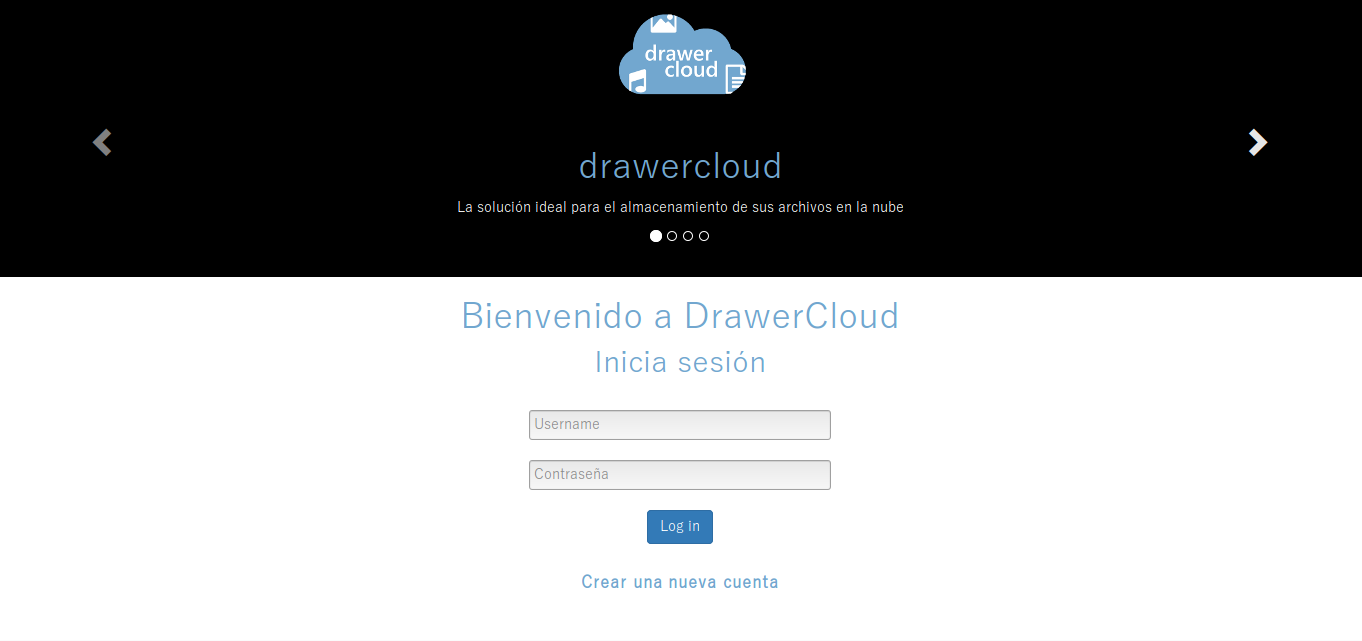
\includegraphics[width=1\textwidth]{imagenes/login}
	\caption{Acceso a la aplicación. Página de login}
	\label{fig:login}
\end{figure}

\begin{figure}[H]
	\centering
	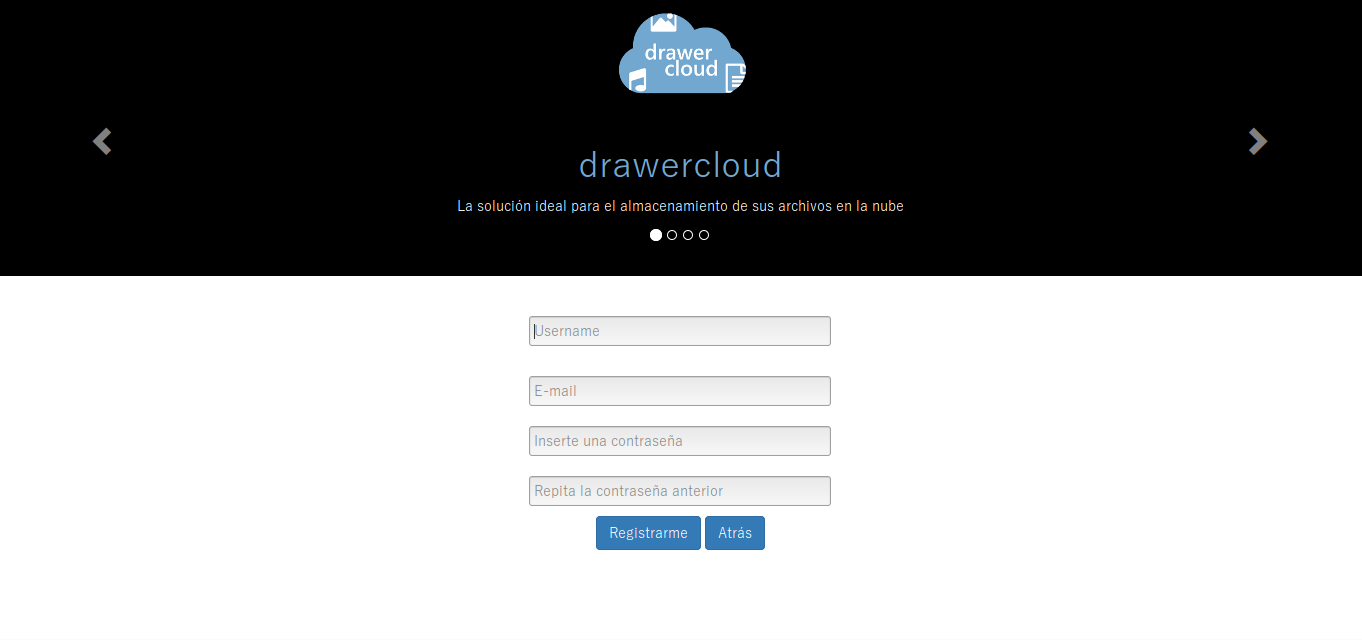
\includegraphics[width=1\textwidth]{imagenes/registro}
	\caption{Acceso a la aplicación. Página de registro}
	\label{fig:registro}
\end{figure}

\section{Página principal - Documentos}
La página principal es la sección \textbf{Documentos} \ref{fig:documentos}. En esta página nos encontraremos con una estructura de directorios y archivos. La vista en que se muestran los directorios y archivos se podrá cambiar haciendo uso de los botones de la imagen \ref{fig:bts_cambiar_vista}, estando disponibles dos tipos de vista: lista \ref{fig:documentos} o iconos \ref{fig:documentos_iconos}.


\begin{figure}[H]
	\centering
	\begin{subfigure}{0.4\textwidth}
		\centering
		
\includegraphics[width=.4\linewidth]{imagenes/bt_cambiar_vista_iconos}
		\caption{Cambiar a la vista \textbf{iconos}}
		\label{fig:bt_cambiar_vista_iconos}
	\end{subfigure}%
	\begin{subfigure}{0.4\textwidth}
		\centering
		
\includegraphics[width=.4\linewidth]{imagenes/bt_cambiar_vista_lista}
		\caption{Cambiar a la vista \textbf{lista}}
		\label{fig:bt_cambiar_vista_lista}
	\end{subfigure}
	\caption{Botones disponibles para cambiar la vista}
	\label{fig:bts_cambiar_vista}
\end{figure}

\begin{figure}[H]
	\centering
	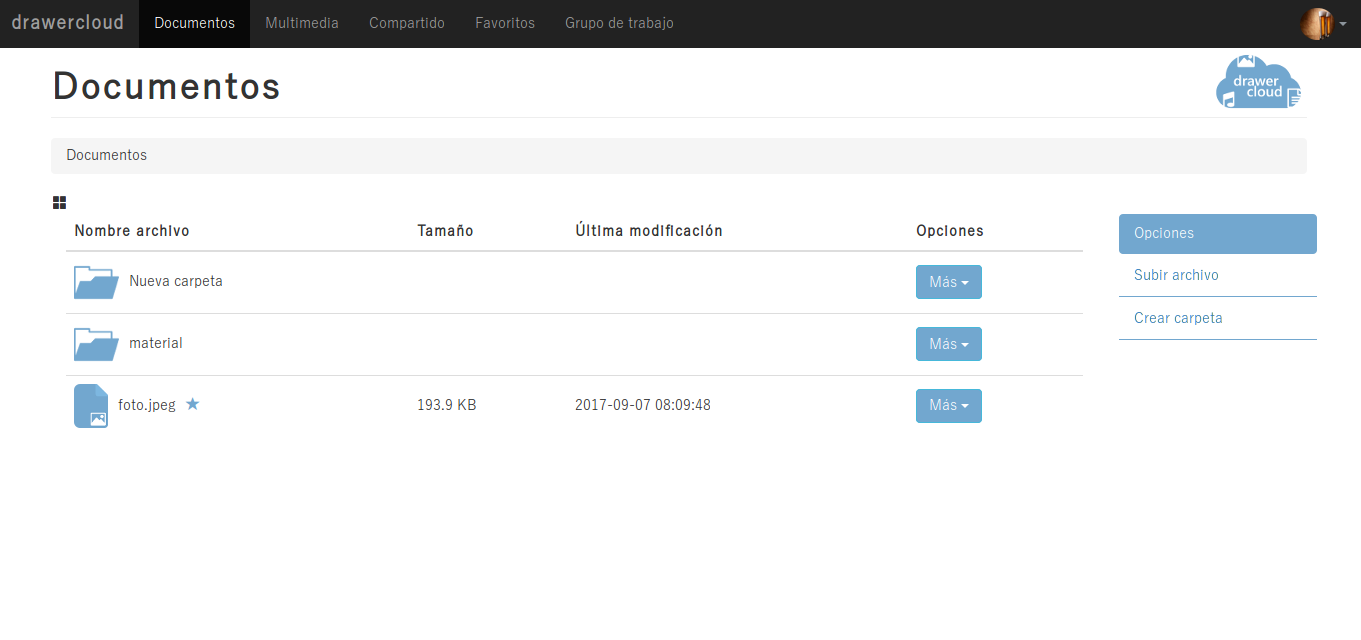
\includegraphics[width=1\textwidth]{imagenes/documentos}
	\caption{Documentos. Aspecto de la página principal}
	\label{fig:documentos}
\end{figure}

\begin{figure}[H]
	\centering
	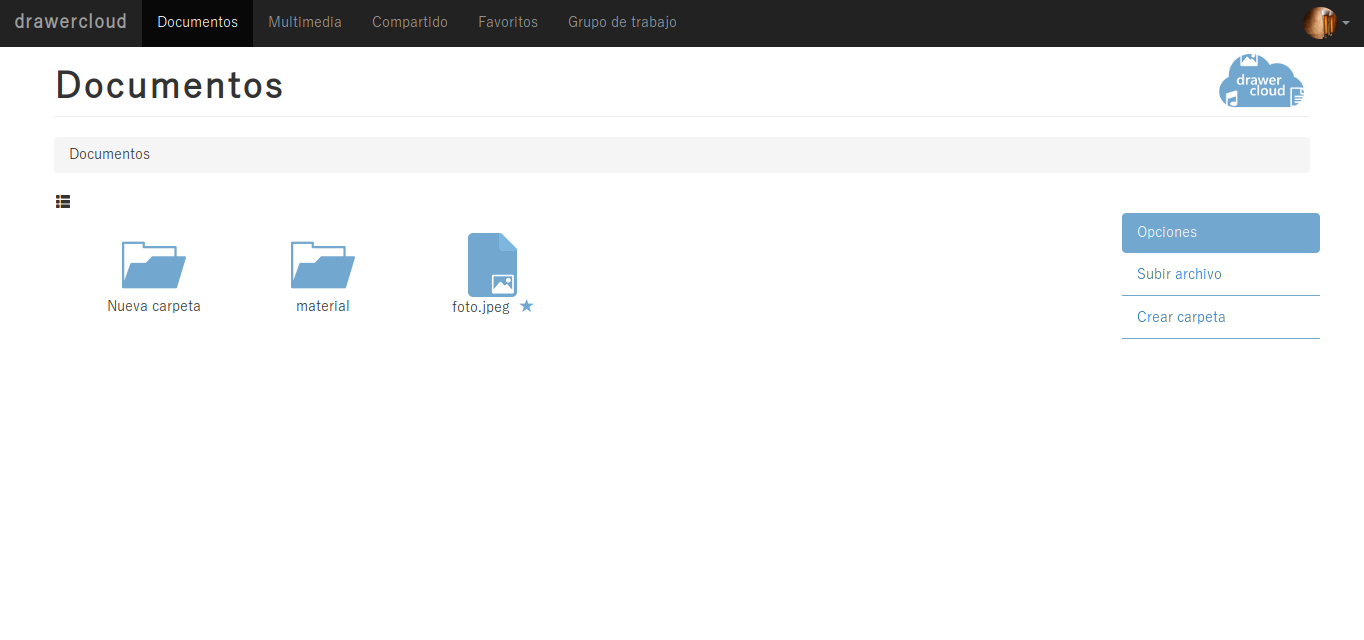
\includegraphics[width=1\textwidth]{imagenes/documentos_iconos}
	\caption{Documentos. Aspecto de la página principal}
	\label{fig:documentos_iconos}
\end{figure}

En \textbf{Documentos} vamos a poder almacenar los archivos que deseemos, podiendo organizar tales archivos en directorios. Para \textbf{crear directorios} o \textbf{subir archivos} hacemos uso de las opciones que aparecen a la derecha de la página documentos \ref{fig:opciones_documentos}.

\begin{figure}[H]
	\centering
	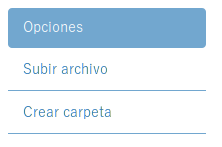
\includegraphics[width=0.4\textwidth]{imagenes/opciones_documentos}
	\caption{Documentos. Opciones de la página Documentos}
	\label{fig:opciones_documentos}
\end{figure}

Los archivos y directorios disponen de \textbf{funcionalidades} propias, como la posibilidad de descargar un archivo, copiar un directorio, etc. Para acceder a estas opciones podemos elegir entre hacer \textbf{click derecho} sobre los directorios/archivos o seleccionar el botón \textbf{Más} disponible para la vista lista.

\subsection{Opciones para archivos}
\begin{itemize}
	\item \textbf{Descargar:}
	\item \textbf{Compartir:}
	\item \textbf{Cambiar nombre:}
	\item \textbf{Copiar en:}
	\item \textbf{Mover a:}
	\item \textbf{Añadir a favoritos:}
	\item \textbf{Eliminar:}
\end{itemize} 

\subsection{Opciones para directorios}
\begin{itemize}
	\item \textbf{Cambiar nombre:}
	\item \textbf{Copiar en:}
	\item \textbf{Mover a:}
	\item \textbf{Eliminar:}
\end{itemize} 